\subsection*{System Track Baselines}

\subsubsection*{Acoustic Scene Classification (ASC)}
\begin{figure}[t]
    \centering
    \begin{subfigure}{0.48\textwidth}
        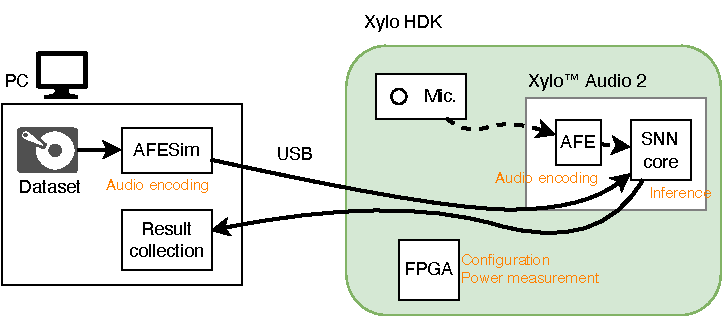
\includegraphics[width=\linewidth]{figures/xylo_system_overview.pdf}
    \vspace*{1cm}
    \end{subfigure}
    \hspace*{0.5cm}
    \begin{subfigure}{0.3\textwidth}
        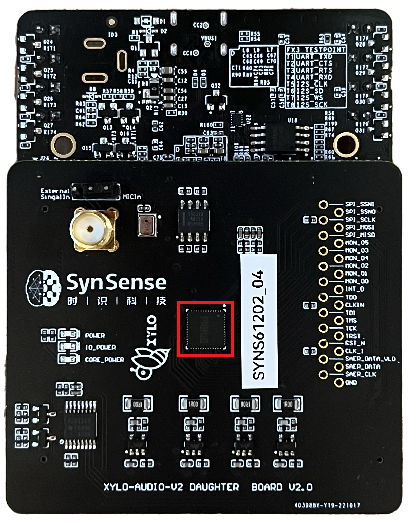
\includegraphics[width=\linewidth]{figures/xyloa2_hdk_fig.pdf}
    \end{subfigure}
        \caption{\secondrev{Left: An overview of the benchmarking system for the Xylo. A simulator of the analog encoding module is run on a PC and streamed to the SNN inference core via USB. After inference, outputs are routed back to the PC for classification. An on-board FPGA configures and records power of the Xylo components. Right: The Xylo\texttrademark Audio 2 hardware development kit (HDK), used as the SUT. The red outline marks the Xylo inference module. Figures taken, with permission, from Ke et al.~\cite{ke2024neurobenchdcase2020acoustic}}}
        \label{fig:xylo}
\end{figure}


\secondrev{\paragraph{CPU} The CPU baseline uses an Arduino Nano 33 BLE board, which runs preprocessing and inference on an ARM Cortex-M4F microcontroller running at 64MHz. All training and deployment uses Edge Impulse, a commercially developed ML-operations platform for tinyML~\cite{hymel2023edgeimpulsemlopsplatform}. The 1 second digital audio samples were converted into two-dimensional frames of Mel-filterbank energies (MFE), and inference uses a network with two convolution layers with batch normalization and max pooling. The trained model was quantized then compiled to an Arduino library using Edge Impulse EON compiler, which optimizes for memory and flash usage. Execution time is measured using on-chip timers from the Arduino, while power is measured using an external multimeter for total system power. Power was measured separately for idle, active pre-processing, and active inference by taking the average power over 60 seconds. The Arduino repeatedly computes over one sample loaded in memory, with a recording frequency of 3 Hz on a Keysight 34465A digital multimeter.}

\secondrev{\paragraph{Synsense Xylo} As shown in Figure~\ref{fig:xylo}, the Xylo baseline used a host PC to run a simulation of the analog pre-processing unit on the benchmark dataset, which was routed into the SNN core on the Xylo SUT. Accuracy is measured by performing a maximum on the output spikes of the SNN. The SNN on Xylo is a feedforward network with three hidden layers, where each layer is connected by synapses with varying time delays. Training is done using the open-source Rockpool toolchain~\cite{rockpool2019}. In order to amortize measurement overheads, power and execution time are measured over continuous streams of 10 seconds of audio, where the execution time result is divided by 10 and the power result is averaged over the duration. The measurements are made by the on-board FPGA, which operates at 12.5MHz and samples power at 1280 Hz. Accuracy is still measured on the 1-second samples. Full details are available in Ke et al.~\cite{ke2024neurobenchdcase2020acoustic}}


\subsubsection*{Quadratic Unconstrained Binary Optimization (QUBO)}
\begin{figure}[t]
    \centering
        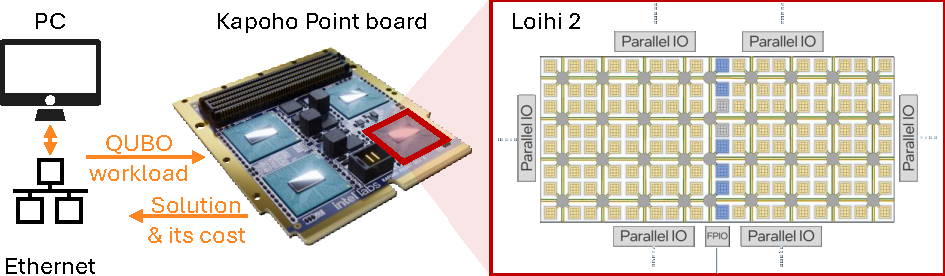
\includegraphics[width=0.85\linewidth]{figures/Loihi2_Benchmarking.pdf}
        \caption{\secondrev{A Kapoho Point board with Loihi 2 chips is connected to a host PC via ethernet. Shown here is a Kapoho Point board with 8 Loihi 2 chips, while the experiments were run on a board with 1 Loihi 2 chip. The QUBO workload is loaded onto the chip, and all processing happens on Loihi 2. On Loihi 2, the neuro-cores, in yellow, are arranged in two $8\times{}8$ grids and iteratively update the variables of the QUBO workload. Embedded CPUs, shown in blue, monitor the cost of the variable assignment. Six parallel IO ports enable 3D stacking of multiple chips for larger workloads than used here. An additional IO port provides the communication to the host PC. The energy and runtime measurements cover the computation of the Loihi 2 chip.}}
        \label{fig:loihi2}
\end{figure}


\secondrev{The processors ran repeatedly with five different initial variable assignments and seeds for different timeouts between $10^{-3}$ s to $10^{3}$ s, and for different workloads sizes of up to $1000$ variables. The neuromorphic algorithm is a parallelized version of simulated annealing that was running on a Kapoho Point board with one Loihi 2 chip, as shown in Figure~\ref{fig:loihi2}. The Loihi 2 board was controlled using Lava \texttt{0.8.0} and Lava Optimization \texttt{0.3.0}. For comparison with conventional hardware, two solvers were adopted based on simulated annealing and tabu search, as implemented in the D-Wave Samplers \texttt{v1.1.0} library \cite{dwavesamplers}. The library was compiled on Ubuntu \texttt{20.04.6 LTS} with GCC \texttt{9.4.0}  and Python \texttt{3.8.10}. CPU measurements were obtained on a machine with Intel Core i9-7920X CPU @ 2.90 GHz and 128GB of DDR4 RAM, using Intel SoC Watch for Linux OS \texttt{2023.2.0}. All details on the solvers, benchmarking routine, and results have been provided by Pierro et al.~\cite{pierro2024solvingquboloihi2}.
}